\documentclass[10pt,twocolumn]{article}
% Form nach A. Suleman, "Optimal lattices for a three-body power-law energy" (Preprint 2026): zweispaltig, Journal-Kopf, Inline-Abstract.
\usepackage[utf8]{inputenc}\usepackage[T1]{fontenc}\usepackage{lmodern}\usepackage{microtype}
\usepackage[english]{babel}\usepackage[a4paper,top=2.3cm,bottom=2.3cm,left=1.8cm,right=1.8cm,columnsep=0.65cm]{geometry}
\usepackage{amsmath,amssymb,amsthm}\usepackage{graphicx}\usepackage{booktabs,array,calc}
\usepackage[font=small,labelfont=bf,labelsep=space,figurename=Fig.]{caption}
\usepackage{fancyhdr}\usepackage{titlesec}\usepackage[hidelinks]{hyperref}\usepackage[capitalise,noabbrev]{cleveref}\usepackage{newunicodechar}
\titleformat{\section}{\normalfont\large\bfseries}{\thesection}{0.6em}{}\titleformat{\subsection}{\normalfont\bfseries}{\thesubsection}{0.6em}{}
\titlespacing*{\section}{0pt}{1.6ex plus .5ex}{0.9ex}\titlespacing*{\subsection}{0pt}{1.2ex plus .4ex}{0.6ex}
\newunicodechar{η}{\ensuremath{\eta}}
\newunicodechar{Δ}{\ensuremath{\Delta}}
\newunicodechar{σ}{\ensuremath{\sigma}}
\newunicodechar{μ}{\ensuremath{\mu}}
\newunicodechar{≥}{\ensuremath{\geq}}
\newunicodechar{≤}{\ensuremath{\leq}}
\newunicodechar{×}{\ensuremath{\times}}
\newunicodechar{→}{\ensuremath{\to}}
\newunicodechar{≈}{\ensuremath{\approx}}
\newunicodechar{−}{\ensuremath{-}}
\newunicodechar{·}{\ensuremath{\cdot}}
\newunicodechar{∈}{\ensuremath{\in}}
\newunicodechar{…}{\ensuremath{\ldots}}
\newunicodechar{²}{\ensuremath{^{2}}}
\newunicodechar{³}{\ensuremath{^{3}}}
\newunicodechar{√}{\ensuremath{\surd}}
\newunicodechar{±}{\ensuremath{\pm}}
\newunicodechar{⁻}{\ensuremath{^{-}}}
\newunicodechar{¹}{\ensuremath{^{1}}}
\newunicodechar{₀}{\ensuremath{_{0}}}
\newunicodechar{₁}{\ensuremath{_{1}}}
\newunicodechar{₂}{\ensuremath{_{2}}}
\newunicodechar{α}{\ensuremath{\alpha}}
\newunicodechar{β}{\ensuremath{\beta}}
\newunicodechar{γ}{\ensuremath{\gamma}}
\newunicodechar{ε}{\ensuremath{\varepsilon}}
\newunicodechar{τ}{\ensuremath{\tau}}
\newunicodechar{ν}{\ensuremath{\nu}}
\newunicodechar{∞}{\ensuremath{\infty}}
\newunicodechar{≠}{\ensuremath{\neq}}
\newunicodechar{π}{\ensuremath{\pi}}
\newunicodechar{λ}{\ensuremath{\lambda}}
\newunicodechar{ρ}{\ensuremath{\rho}}
\newunicodechar{θ}{\ensuremath{\theta}}

\sloppy\emergencystretch=1.5em
\providecommand{\tightlist}{\setlength{\itemsep}{0pt}\setlength{\parskip}{0pt}}
\newtheorem{theorem}{Theorem}\newtheorem{conjecture}{Conjecture}\newtheorem{proposition}{Proposition}\newtheorem{lemma}{Lemma}\newtheorem{corollary}{Corollary}
\theoremstyle{definition}\newtheorem{definition}{Definition}\newtheorem{example}{Example}
\newtheorem{observation}{Numerical observation}\theoremstyle{remark}\newtheorem{remark}{Remark}
\pagestyle{fancy}\fancyhf{}\renewcommand{\headrulewidth}{0pt}
\fancyhead[L]{\small Preprint (2026)}\fancyhead[R]{\small N. Schittenhelm: Closed forms for the constants in the odd-weight identities ...}\fancyfoot[C]{\small\thepage}
\begin{document}
\twocolumn[{%
\noindent{\small Preprint}\\[-1pt]
\noindent{\small\itshape Mathematical Physics}\\[12pt]
\noindent{\LARGE\bfseries\raggedright Closed forms for the constants in the odd-weight identities between dihedral modular graph functions\par}\vspace{10pt}
\noindent{\large Noah Schittenhelm}\\[3pt]
\noindent{\small Hack-Nation 2026, Team Ninja Turtles}\\[2pt]
\noindent{\small Preprint, October 2026}\par\vspace{16pt}
}]
\thispagestyle{plain}
\noindent\textbf{Abstract} Dihedral modular graph functions \(C(a,b,c)\) of weight \(w=a+b+c\) are the coefficients of the low-energy expansion of the one-loop closed-string amplitude. For each odd weight there is a combination \(X_w\) whose Laplacian is a multiple of \(E(w)\). We determine the constants in \(X_w = f_w E(w) + g_w \zeta(w)\). Theorem 1 gives \(f_w = 3((w-1)/2)!/w\) and \(g_w = 6|B_{w-1}|/((w-1)/2)!\) for the odd weights \(3 \le w \le 61\) examined. The proof combines exact rational Laplace algebra, a harmonicity argument and the Laurent constant term evaluated in rational arithmetic. It rests on two assumptions that were not machine-checked: a published theorem on Laurent polynomials and a standard lemma. Theorem 2 shows exactly, for the weights \(3 \le w \le 25\) examined, that the space of combinations with \(\Delta X \in \mathbb{Q}\,E(w)\) has dimension 1 for odd \(w\) and 0 for even \(w\). Independent numerical confirmation at 32 digits covers \(w = 3, 5, 7, 9, 11, 13, 15, 17\), with \(w = 15\) a prediction and \(w = 17\) a preregistered blind test. The full weight-11 basis has exactly one relation numerically. A proof beyond the examined range is stated as a conjecture and remains open.
\par\medskip
\noindent\textbf{Keywords} Modular graph functions $\cdot$ Laplace eigenvalue equations $\cdot$ Eisenstein series $\cdot$ Bernoulli numbers $\cdot$ Genus-one string amplitudes $\cdot$ Computer-assisted proof\par\medskip
\textbf{Noah Schittenhelm} (Hack-Nation, Team Ninja Turtles)

\section{Introduction}\label{introduction}

Two-loop modular graph functions \(C(a,b,c)\) satisfy Laplace eigenvalue equations with inhomogeneous terms that are polynomial in non-holomorphic Eisenstein series \cite{DHoker20156698}. D'Hoker, Green and Vanhove (DGV) obtained, for each odd weight, a combination \(X_w\) that is annihilated by the Laplacian after subtracting a multiple of \(E(w)\). The remaining additive constant of integration is fixed by the asymptotics at the cusp \cite{DHoker20156698}. DGV give \(f_w\) for \(w\le 9\) and \(g_w\) for \(w=3\) and \(w=5\), while \(g_7\) and \(g_9\) remain undetermined there. The value of \(g_7\) appears explicitly in later work \cite{Dorigoni20215017}.

\textbf{Open question.} What are the exact closed forms of \(f_w\) and \(g_w\) for general odd \(w\)?

\textbf{Why it is hard.} The constant is the \(\tau_2^0\) term of a Laurent polynomial. That polynomial is known for each single \(C_{u,v;w}\), but evaluating it for the DGV combination requires exact bookkeeping of growing coefficient lists. Numerical relation searches are limited by the coefficient height; for the full weight-11 basis the originally preregistered completeness criterion was failed.

\textbf{Contribution.} We evaluate the Laurent constant of \(X_w\) exactly for the odd weights \(3 \le w \le 61\) examined, obtain closed forms, and confirm them independently by numerics.

\textbf{Summary of results.}

\begin{itemize}
\item
  Theorem 1 shows \(X_w = f_w E(w) + g_w \zeta(w)\) with \(f_w = 3((w-1)/2)!/w\) and \(g_w = 6|B_{w-1}|/((w-1)/2)!\) for the odd weights \(3 \le w \le 61\) examined (exact Laplace algebra plus Laurent constant in rational arithmetic).
\item
  Theorem 2 shows that the space \(\{X : \Delta X \in \mathbb{Q}E(w)\}\) has dimension 1 for odd \(w\) and 0 for even \(w\), for the weights \(3\le w\le 25\) examined.
\item
  Numerical results, independent of the proof, confirm the constants at \(w = 3, 5, 7, 9, 11, 13, 15, 17\) and show that the full weight-11 basis has exactly one relation.
\end{itemize}

\section{Setting}\label{setting}

Let \(\tau=\tau_1+i\tau_2\), \(q=e^{2\pi i\tau}\) and \(p=m\tau+n\). The lattice sums use the normalisation \((\tau_2/(\pi|p|^2))^a\):

Here \((a_1,a_2,a_3)=(a,b,c)\) and \(w=a+b+c\). \(\zeta(k)\) is the Riemann zeta value and \(B_n\) are Bernoulli numbers. The Laplacian is \(\Delta=\tau_2^2(\partial_{\tau_1}^2+\partial_{\tau_2}^2)\). \(E(w)\) is an eigenfunction, \(\Delta E(w)=w(w-1)E(w)\). For odd \(w\), \(X_w\) is the DGV combination (eq. 3.57), normalised so that \(\Delta X_w=w(w-1)f_wE(w)\).

Numerical parameters of the verifier:

\begin{itemize}
\tightlist
\item
  four random points, seed 4711, with \(|\tau_1|\le 1/2\) and \(1\le\tau_2\le 2.5\);
\item
  working precision of 32 digits;
\item
  tolerance 1e-24 for relative residuals, and 1e-14 when a Laplacian is involved;
\item
  fourth-order finite-difference Laplacian with step \(h=\) 1e-6.
\end{itemize}

\section{Closed forms for odd weight}\label{closed-forms-for-odd-weight}

\begin{theorem}[Closed forms, $w\le 61$]
For the odd weights \(3\le w\le 61\) examined,
\[X_w=f_wE(w)+g_w\zeta(w),\quad f_w=\frac{3((w-1)/2)!}{w},\quad g_w=\frac{6|B_{w-1}|}{((w-1)/2)!}\quad\text{}\]
\end{theorem}

\emph{Proof.} The proof has three steps and a fourth that supplies the constant.

\begin{enumerate}
\def\labelenumi{\arabic{enumi}.}
\tightlist
\item
  Exact rational computation in the algebraic Laplace representation gives \(\Delta X_w=w(w-1)f_wE(w)\) with no other terms. Since \(\Delta E(w)=w(w-1)E(w)\), it follows that \(\Delta(X_w-f_wE(w))=0\).
\item
  \(X_w-f_wE(w)\) is \(SL(2,\mathbb{Z})\)-invariant and of polynomial growth at the cusp. By the standard argument used by DGV it is therefore constant.
\item
  The constant is the \(\tau_2^0\) term of the Laurent polynomial of \(X_w\). It was computed in rational arithmetic from Proposition 2.1 and Theorem 5.1 of D'Hoker-Kaidi, with the transcription checked against their eq. 5.19. All Laurent terms not involving products of zeta values agree with those of \(f_wE(w)+g_w\zeta(w)\) (consistency check). The constant equals \(g_w\zeta(w)\) with \(g_w=6|B_{w-1}|/((w-1)/2)!\) for the odd weights \(3\le w\le 61\) examined.
\end{enumerate}

Assumptions not checked by code are the correctness of Theorem 5.1 of D'Hoker-Kaidi and the standard lemma in step 2. Theorem 5.1 is proved there in its Appendix A; its conjectural part concerns only the coefficient of \(\tau_2^{2-w}\) and is not used. Examples are \(g_3=1\), \(g_5=1/10\), \(g_7=1/42\), \(g_9=1/120\).

Novelty status: partly known. Closed forms of \(f_w\) and \(g_w\) for general odd \(w\) and their proof for \(w\ge 9\) are not given there.

\begin{table}[t]\centering\footnotesize
\caption{Constants \(f_w\) and \(g_w\) in \(X_w=f_wE(w)+g_w\zeta(w)\) (DGV normalisation of \(X_w\)), exact for odd \(3\le w\le 25\).}
\begin{tabular}{@{}lll@{}}
\toprule
\(w\) & \(f_w\) & \(g_w\) \\
\midrule
3 & 1 & 1 \\
5 & 6/5 & 1/10 \\
7 & 18/7 & 1/42 \\
9 & 8 & 1/120 \\
11 & 360/11 & 1/264 \\
13 & 2160/13 & 691/327600 \\
15 & 1008 & 1/720 \\
17 & 120960/17 & 3617/3427200 \\
19 & 1088640/19 & 43867/48263040 \\
21 & 518400 & 174611/199584000 \\
23 & 119750400/23 & 77683/83462400 \\
25 & 57480192 & 236364091/217945728000 \\
\bottomrule
\end{tabular}
\end{table}


\section{Uniqueness of the harmonic combination}\label{uniqueness-of-the-harmonic-combination}

\begin{theorem}[Dimension of the harmonic space]
For odd \(w\) it is spanned by the DGV combination, with \(\Delta X=w(w-1)f_wE(w)\) and \(f_w=3((w-1)/2)!/w\).
\end{theorem}

\emph{Certificate.} The statement was verified exactly for the weights \(3\le w\le 25\) examined, with the algebraic Laplace representation of DGV, re-derived and evaluated in rational arithmetic. Novelty status: partly known. The one-dimensionality of the eigenspace for odd weight, its vanishing for even weight and the combination \(X_w\) are known.

\begin{proposition}[Laplace equations at $w=9$ and $w=11$]
\(\Delta\big(9C(4,4,1)+18C(4,3,2)+4C(3,3,3)\big)=288\,E(9)\) and \(\Delta\big(2C(5,5,1)+4C(5,4,2)+2C(5,3,3)+3C(4,4,3)\big)=100\,E(11)\).
\end{proposition}

\emph{Certificate.} Both equations were obtained in the algebraic Laplace representation and checked in exact rational arithmetic. The verifier returns a single value of \(\lambda\) in \(\Delta X=\lambda E(w)\). Novelty status: the \(w=9\) equation is already known. For \(w=11\) the combination is known, but \(f_w\) and \(g_w\) are not given there.

\begin{conjecture}[Beyond the examined range]
The identity \(X_w=f_wE(w)+g_w\zeta(w)\) with the closed forms of Theorem 1 holds beyond the examined range of odd weights.
\end{conjecture}

Before the proof, this was a conjecture read off from \(w = 3..13\).

\section{Numerical confirmation, independent of the proof}\label{numerical-confirmation-independent-of-the-proof}

The statements in this section are numerical (32 digits, four verifier-chosen points) combined with the exact vanishing of the leading Laurent coefficient. They do not use the proof of Theorem 1.

\begin{example}[Weight 3]
\(C(1,1,1)-E(3)-\zeta(3)=0\) as functions of \(\tau\).
\end{example}

\emph{Certificate.} The exact leading Laurent coefficient in \(y^3\) vanishes, and at the four verifier points the maximal relative residual is 5.13e-44 against the bound 1e-24. This identity is already known \cite{DHoker20156698}.

\begin{example}[Weight 5]
\(30\,C(2,2,1)-12\,E(5)-\zeta(5)=0\) as functions of \(\tau\).
\end{example}

\emph{Certificate.} The leading coefficient in \(y^5\) vanishes exactly, and the maximal relative residual is 1.57e-43. This identity is already known \cite{DHoker20156698}.

\begin{example}[Weight 7]
\(252\,C(3,3,1)+252\,C(3,2,2)-108\,E(7)-\zeta(7)=0\) as functions of \(\tau\).
\end{example}

\emph{Certificate.} The leading coefficient in \(y^7\) vanishes exactly, and the maximal relative residual is 1.59e-43. This is \(f_7\) and \(g_7\) in the notation above, already known \cite{Dorigoni20215017}.

\begin{observation}[Weight 9]
\(960\,E(9)+\zeta(9)-2160\,C(4,4,1)-4320\,C(4,3,2)-960\,C(3,3,3)=0\) as functions of \(\tau\).
\end{observation}

\emph{Certificate.} The leading coefficient in \(y^9\) vanishes exactly, and the maximal relative residual is 8.33e-44. Novelty status: partly known. DGV give the identity with an undetermined constant \(g_9\), whose value is not given there.

Here \(E(w)\) is the lattice sum of the Setting and \(\zeta(w)\) the Riemann zeta value at \(w\).

\begin{table}[t]\centering\footnotesize
\caption{Numerical checks of the integer-normalised relations at weights 11, 13, 15, 17; the third column is the maximal relative residual at the four verifier points (bound 1e-24).}
\begin{tabular}{@{}lll@{}}
\toprule
\(w\) & coefficients of \(E(w)\) and \(\zeta(w)\) & residual \\
\midrule
11 & \(-8640\,E(11)\), \(-\zeta(11)\) & 1.21e-43 \\
13 & \(-54432000\,E(13)\), \(-691\,\zeta(13)\) & 5.67e-44 \\
15 & \(-725760\,E(15)\), \(-\zeta(15)\) & 6.46e-44 \\
17 & \(-24385536000\,E(17)\), \(-3617\,\zeta(17)\) & 5.49e-44 \\
\bottomrule
\end{tabular}
\end{table}


Each of the four relations has vanishing exact leading Laurent coefficient (in \(y^{11}\), \(y^{13}\), \(y^{15}\), \(y^{17}\)). The value at \(w = 15\) was a prediction made before its value was read, and \(w = 17\) was a preregistered blind test. Novelty status: partly known. Existence and combination for each odd \(w\) are known, but \(f_w\) and \(g_w\) for \(w\ge 11\) are not given there.

\begin{observation}[Full weight-11 basis]
The rational linear relations among \(C(9,1,1)\), \(C(8,2,1)\), \(C(7,3,1)\), \(C(7,2,2)\), \(C(6,4,1)\), \(C(6,3,2)\), \(C(5,5,1)\), \(C(5,4,2)\), \(C(5,3,3)\), \(C(4,4,3)\), \(E(11)\), \(\zeta(11)\) form a space of dimension exactly 1 (weight 11), spanned by the weight-11 relation of the table.
\end{observation}

The threshold was chosen so as to separate the null value 1.11e-43 from the smallest large singular value 3.69e-9. One singular value is below 1e-24 and 11 are above 1e-16. Novelty status: partly known; see the weight-11 entry above.

\begin{observation}[Hardening of the weight-11 identity]
An independent direct lattice summation in double precision agrees to at most 1e-12 relative at 8 of 8 points.
\end{observation}

\emph{Certificate.} The criterion operationalises the preregistered expectation that the residual decreases with precision; an exact 0 counts as below rounding resolution. The run exposed and fixed an evaluator bug. The Fourier sum for \(E_s\) stopped when a term vanished, which happens at \(\tau_1=1/4\) where \(\cos(2\pi N\tau_1)=0\) for odd \(N\). Before the fix that point showed a precision-independent residual of 3.5e-10. All listed points were computed with the corrected code, and no earlier test point was affected.

\begin{remark}[Status of the computer-assisted parts]
The trusted base consists of the following.

\begin{itemize}
\tightlist
\item
  \textbf{Exact rational arithmetic.} It covers the Laplace algebra of Theorems 1 and 2 and the Laurent constants.
\item
  \textbf{The 32-digit evaluator.} It covers the numerical observations, with the tolerances of the Setting.
\end{itemize}

Not machine-checked are Theorem 5.1 of D'Hoker-Kaidi and the harmonic-implies-constant lemma. A third party re-runs all certificates with the commands in the Declarations. Statements marked numerical are not proofs.
\end{remark}

\section{Discussion}\label{discussion}

\textbf{Limitations.} The proof depends on two external ingredients, listed in the status remark. The range \(w\le 61\) is a computational bound, not a theorem beyond it. Numerical confirmation certifies values at sampled points together with exact leading coefficients, for the weights \(w = 3, 5, 7, 9, 11, 13, 15, 17\) examined.

\textbf{What did not work.}

It was reported openly, and criterion 2, preregistered afterwards on new data, passed.
- The hardening run found an evaluator bug at \(\tau_1=1/4\) (early termination of the Fourier sum when a term vanished). It was fixed, and all listed points use the corrected code.

Further negative results are collected in Appendix A.

\textbf{Open questions.}

\begin{enumerate}
\def\labelenumi{(\roman{enumi})}
\item
  Is there a proof of \(X_w=f_wE(w)+g_w\zeta(w)\) beyond the examined range, i.e.~of Conjecture 1, presumably via a binomial-sum identity for the Laurent constant?
\item
  What are the constants in the non-harmonic Laplace eigenvalue equations for \(C(a,b,c)\)?
\item
  Do analogous closed forms exist at higher loop order?
\end{enumerate}

\section*{Declarations}\label{declarations}
\addcontentsline{toc}{section}{Declarations}

\textbf{Affiliation} Noah Schittenhelm, Hack-Nation, Team Ninja Turtles.

\textbf{Acknowledgements} Computations, literature searches and parts of the manuscript were prepared with an automated verifier-gated laboratory built on the AI system Claude (Anthropic). Every statement was accepted only after verification by code. The authors are responsible for the content.

\textbf{Code and data availability} Repository https://github.com/NinjaTurtlesHackathons/Hacknation, branch \texttt{claude/modulformen-paper}, directory \texttt{projects/modular}. All certificates are reproduced with \texttt{python\ -m\ asd.recheck\ modular}, and the paper is rebuilt with \texttt{python\ -m\ asd.paper\ -\/-domain\ modular}.

\textbf{Competing interests} None.

\appendix

\section{Numerical methods and error control}\label{numerical-methods-and-error-control}

\textbf{Certificate types.}

\begin{enumerate}
\def\labelenumi{\arabic{enumi}.}
\tightlist
\item
  \emph{Exact Laplace algebra and Laurent constants:} rational arithmetic, no floating point.
\item
  \emph{Function relations:} the leading Laurent coefficient is checked exactly, then numerically at four verifier points (seed 4711, 32 digits, tolerance 1e-24, or 1e-14 with the finite-difference Laplacian of step 1e-6).
\item
  \emph{Relation spaces:} completeness is shown by a singular-value gap of the normalised value matrix at independent points (seed 4712).
\end{enumerate}

\textbf{Validation of the verifier on known results.}

The singular values of the normalised matrices show one value below 1e-24; for \(w = 3\) the matrix is 6x3 with smallest large value 0.731.
- Laplace equations: \(\Delta C(3,1,1)-6C(3,1,1)-\tfrac{86}{5}E(5)+4E(2)E(3)-\tfrac1{10}\zeta(5)=0\) with residual 1.63e-25. \(\Delta C(2,1,1)-2C(2,1,1)-9E(4)+E(2)^2=0\) with 2.39e-25. \(\Delta C(2,2,1)-8E(5)=0\) with 6.99e-26. \(\Delta C(2,2,1)-20C(2,2,1)+\tfrac23\zeta(5)=0\) with 6.74e-26.
- Holomorphic identities (exact, Sturm certificates):
- \(\theta(1)^4=\eta(2)^{20}\eta(1)^{-8}\eta(4)^{-8}\) on \(\Gamma_0(4)\), with coefficients \(q^0..q^{11}\) vanishing and Sturm bound 1. The weight-1 version \(\theta(1)^2=\eta(2)^{10}\eta(1)^{-4}\eta(4)^{-4}\) also holds. The relation of eta quotients to theta functions is stated in \cite{Vasuki202671v1}.
- \(\theta_{\mathrm{E8}}=E_4\), \(\theta_{\mathrm{E8}}^2=\theta_{\mathrm{D16}}\), \(\theta_{\mathrm{E8}}^2=E_4^2\) and \(\theta_{\mathrm{E8}}^2=E_8\).
- \(1728\,\Delta=E_4^3-E_6^2\), a classical fact stated in \cite{Jorgenson201542v1}, and \(j\Delta=E_4^3\).
- Eta quotients with trivial character span \(M_4(\Gamma_0(N))\) exactly for \(N\in\{2, 4, 5, 6, 8, 9, 10, 12, 14, 15, 16, 18, 20, 22, 24, 25, 26, 27, 28, 30\}\) and not for \(N\in\{1, 3, 7, 11, 13, 17, 19, 21, 23, 29\}\) (exact, exhaustive, \(N\le 30\)).

\textbf{Negative results.}

\begin{itemize}
\tightlist
\item
  At weight 6, no claim passed for the relation space of \(C(4,1,1)\), \(C(3,2,1)\), \(C(2,2,2)\) and products of Eisenstein series and zeta values; the 12x9 matrix showed 8 singular values above 1e-8 and none below 1e-24.
\item
  No claim passed for the eta-span table in the first attempts.
  The run was aborted, and the presumed cause is precision too low relative to the coefficient height.
\item
  No claim passed in the first attempt at the weight-13 and weight-15 constants. Both relations were later confirmed.
\end{itemize}

\textbf{Laboratory workflow.} The laboratory ran 17 rounds with 37 verified statements and 4 negative results. Every round was preregistered before the experiment. Statements were proposed by agents in the roles \emph{sparsam}, \emph{numeriker}, \emph{skeptiker} and \emph{theoretiker}, and accepted only if the verifier passed them. Adversarial counter-checks (red team) numbered 53 in total; 4 passed without contradicting the statement, 48 did not pass, and 1 was not executable. The verifier rejected falsified variants, such as a doubled \(\zeta(17)\) coefficient or a wrong \(\zeta(5)\) source term.

\section{Provenance of the statements}\label{provenance-of-the-statements}

The provenance table mapping every statement to its evidence follows (it is generated automatically).

{\def\LTcaptype{none} % do not increment counter
\begin{table*}[t]\centering\footnotesize
\begin{tabular}{@{}
  >{\raggedright\arraybackslash}p{(\linewidth - 2\tabcolsep) * \real{0.5000}}
  >{\raggedright\arraybackslash}p{(\linewidth - 2\tabcolsep) * \real{0.5000}}@{}}
\toprule
\begin{minipage}[b]{\linewidth}\raggedright
Statement
\end{minipage} & \begin{minipage}[b]{\linewidth}\raggedright
Level
\end{minipage} \\
\midrule
Section: Introduction & computed\_rigorous, observed \\
Section: Setting & computed\_rigorous \\
Theorem 1 (Closed forms, \(w\le 61\)) & computed\_rigorous \\
Section: Closed forms for odd weight & computed\_rigorous \\
Theorem 2 (Dimension of the harmonic space) & computed\_rigorous \\
Section: Uniqueness of the harmonic combination & computed\_rigorous \\
Proposition 1 (Laplace equations at \(w=9\) and \(w=11\)) & computed\_rigorous \\
Conjecture 1 (Beyond the examined range) & computed\_rigorous \\
Section: Numerical confirmation, independent of the proof & computed\_rigorous, observed \\
Example 1 (Weight 3) & observed \\
Example 2 (Weight 5) & observed \\
Example 3 (Weight 7) & observed \\
Observation 1 (Weight 9) & observed \\
Observation 2 (Full weight-11 basis) & observed \\
Observation 3 (Hardening of the weight-11 identity) & observed \\
Remark 1 (Status of the computer-assisted parts) & computed\_rigorous, observed \\
Section: Discussion & computed\_rigorous, observed \\
Section: Declarations & observed \\
Section: Appendix A: Numerical methods and error control & computed\_rigorous, observed \\
\bottomrule
\end{tabular}
\end{table*}

}

The complete automatic checking protocol of the writing process is stored as pruefprotokoll.json in the project directory of the repository.

\begin{figure}[t]\centering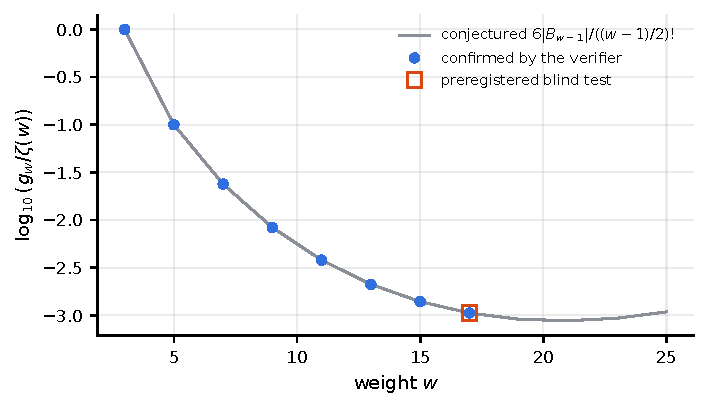
\includegraphics[width=\columnwidth]{konstanten.pdf}\caption{Integration constants $g_w$ of the odd-weight identities in the normalisation of eq. (3.57) of D'Hoker-Green-Vanhove: conjectured closed form (line) and the weights at which the verifier confirmed the identity numerically (dots, 32 digits, 4 verifier points); the square marks the preregistered blind test at $w = 17$.}\end{figure}
\begin{figure}[t]\centering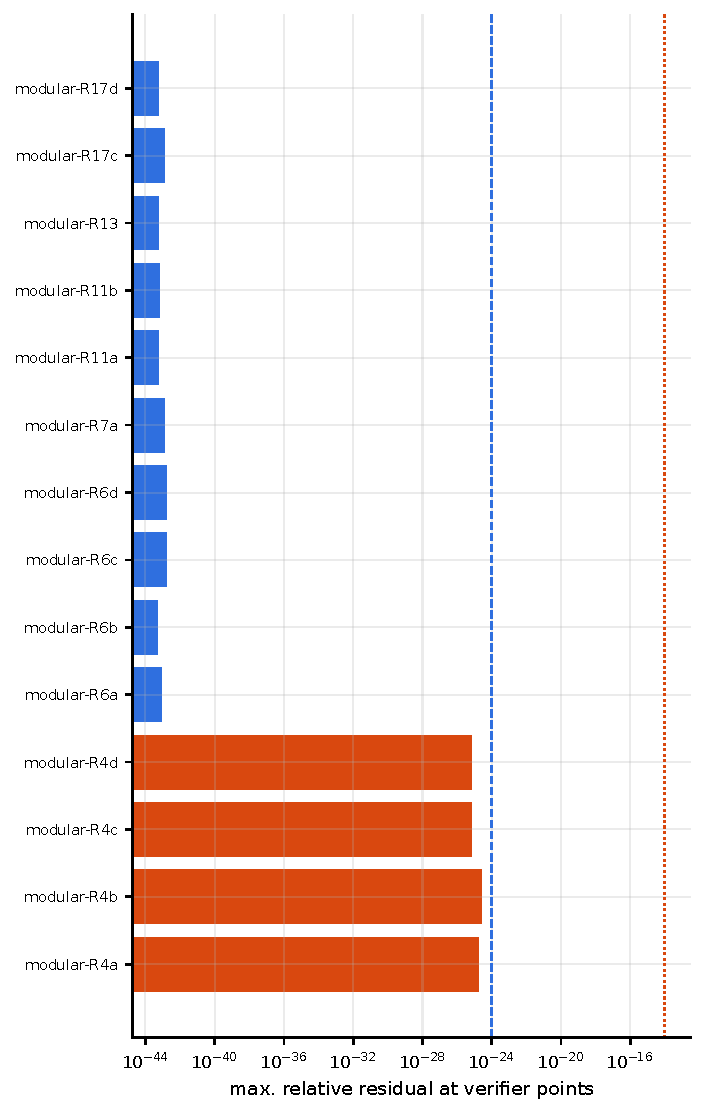
\includegraphics[width=\columnwidth]{margins.pdf}\caption{Numerical verification margins: largest relative residual of each confirmed relation among modular graph functions at the verifier's own random points (32 digits). Dashed: acceptance threshold $10^{-24}$; dotted: threshold $10^{-14}$ for relations containing a Laplacian (orange).}\end{figure}
\begin{figure}[t]\centering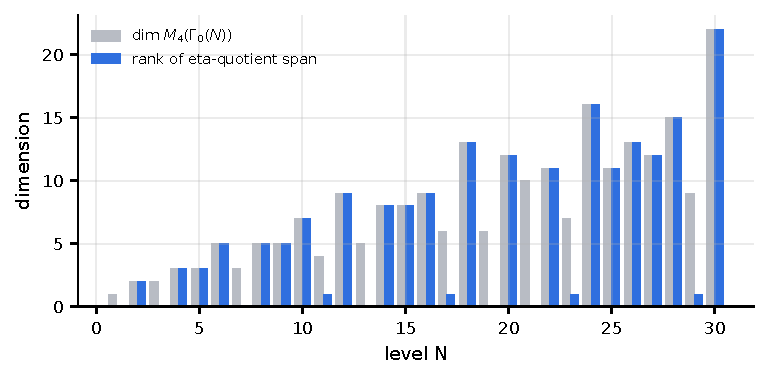
\includegraphics[width=\columnwidth]{eta_span.pdf}\caption{Exact comparison, for every level $N \le 30$, of $\dim M_4(\Gamma_0(N))$ (grey) with the rank of the span of all holomorphic eta quotients of weight 4 with trivial character (blue).}\end{figure}

\bibliographystyle{unsrt}
\bibliography{references}
\end{document}
